\setcounter{section}{2}

\Needspace{5\baselineskip}
\hypertarget{controlling-generation}{%
\section{Controlling Generation}\label{controlling-generation}}

\Needspace{5\baselineskip}
\hypertarget{i.-temperature}{%
\subsection{I. Temperature}\label{i.-temperature}}

\begin{itemize}
\tightlist
\item
  \textbf{High temperature (such as 1.0):} increases diversity in generated results but may make them unstable.
\item
  \textbf{Low temperature (such as 0.1):} produces more stable results but may lack creativity.
\end{itemize}

Temperature controls randomness in generation. Specifically, the parameter \(T\) affects the ``sharpness'' of the probability distribution. Higher temperature produces a smoother distribution and more diverse results; lower temperature produces a sharper distribution and more stable results.

\[
P(x_{T+1} \mid x_1, x_2, \ldots, x_T) =
\frac{\exp\left(\frac{f(x_1,x_2,\ldots,x_T)}{T}\right)}
{\sum_i \exp\left(\frac{f_i(x_1,x_2,\ldots,x_T)}{T}\right)}
\]

Here, \(f(x_1,x_2,\ldots,x_T)\) is the model's internal function, usually a complex neural network such as a Transformer. \(T\) is the temperature parameter, controlling the smoothness of the probability distribution.

\Needspace{5\baselineskip}
\hypertarget{ii.-sampling-token-search-strategies}{%
\subsection{II. Sampling (Token Search) Strategies}\label{ii.-sampling-token-search-strategies}}

\Needspace{5\baselineskip}
\hypertarget{greedy-search}{%
\subsubsection{Greedy Search}\label{greedy-search}}

Always select the most probable next word. The output is stable but may be monotonous.

\[
x_{T+1} = \arg\max P(x_{T+1} \mid x_1, x_2, \ldots, x_T)
\]

Greedy-search example: the image shows a tree starting from ``The,'' selecting the highest-probability branch at each step, such as The -\textgreater{} nice (0.5) -\textgreater{} woman (0.4) \ldots{}

\begin{figure}[htbp]
\centering
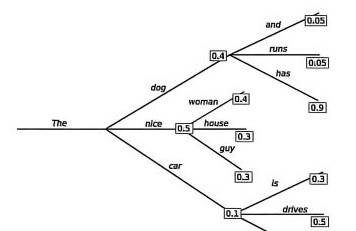
\includegraphics{images/image-0019.jpeg}
\caption{Greedy-search tree example}
\end{figure}

Problem: choosing the largest probability at every step does not guarantee the largest product!

\Needspace{5\baselineskip}
\hypertarget{beam-search}{%
\subsubsection{Beam Search}\label{beam-search}}

Beam search retains the \texttt{num\_beams} most likely words at each time step and ultimately chooses the most probable sequence, reducing the risk of losing potentially high-probability sequences.

Beam-search example: the image shows a tree-search process. Unlike greedy search, it keeps multiple paths at every step, such as ``The nice'' and ``The dog,'' and continues expanding them.

\begin{figure}[htbp]
\centering
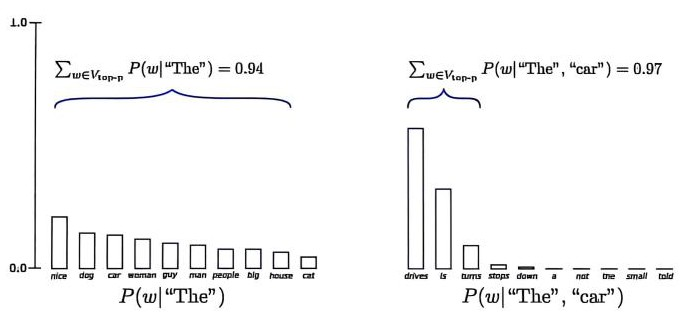
\includegraphics{images/image-0020.jpeg}
\caption{Beam-search tree example}
\end{figure}

\textbf{Top-k sampling:} randomly select the next word from the \(k\) most probable words, balancing stability and diversity.

\[
S_k = \{x_i \mid P(x_i \mid x_1, x_2, \ldots, x_T) \text{ is among the top } k \text{ probabilities}\}
\]

\[
x_{T+1} \sim P(x_{T+1} \mid x_1, x_2, \ldots, x_T) \text{, sampled within } S_k
\]

\textbf{Top-p, or nucleus, sampling:} randomly select the next word from the smallest set whose cumulative probability reaches \(p\), dynamically adjusting the sampling range.

\[
S_p = \{x_i \mid \sum_{j=1}^{i} P(x_j \mid x_1, x_2, \ldots, x_T) \le p\}
\]

\[
x_{T+1} \sim P(x_{T+1} \mid x_1, x_2, \ldots, x_T) \text{, sampled within } S_p
\]

\Needspace{5\baselineskip}
The following diagram illustrates top-p sampling:

\begin{figure}[htbp]
\centering
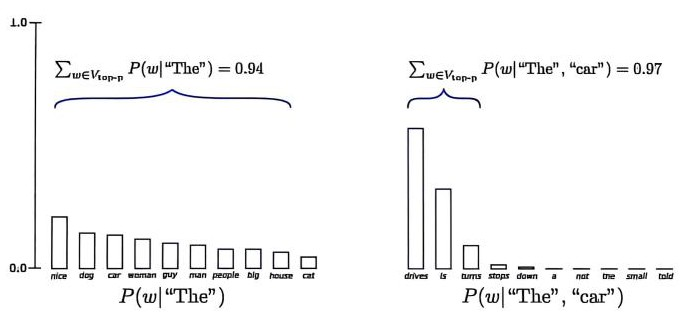
\includegraphics{images/image-0021.jpeg}
\caption{Diagram of a top-p sampling distribution}
\end{figure}

Top-k and top-p can also be combined: first select K words, then select by probability p within that set.

\FloatBarrier
\Needspace{5\baselineskip}
\hypertarget{references-75}{%
\subsection{References}\label{references-75}}

\vspace{0.25em}
\begin{itemize}
\tightlist
\item
  温睦宁、林江浩、张伟楠、俞勇 (2025). \href{https://haa.boyuai.com/}{\emph{Hands-on Learning of Large-Model Agents} (translated title; in Chinese)}. Posts \& Telecom Press. ISBN 978-7-115-68638-1.
\item
  Holtzman, A., Buys, J., Du, L., Forbes, M., \& Choi, Y. (2020). \href{https://arxiv.org/abs/1904.09751}{The Curious Case of Neural Text Degeneration}. ICLR 2020.
\end{itemize}

\clearpage
